\documentclass[12pt,english]{article}
\usepackage{mathptmx}

\usepackage{color}
\usepackage[dvipsnames]{xcolor}
\definecolor{darkblue}{RGB}{0.,0.,139.}

\usepackage[top=1in, bottom=1in, left=1in, right=1in]{geometry}

\usepackage{amsmath}
\usepackage{amstext}
\usepackage{amssymb}
\usepackage{setspace}
\usepackage{indentfirst}

\usepackage[authoryear]{natbib}
\usepackage{url}
\usepackage{booktabs}
\usepackage[flushleft]{threeparttable}
\usepackage{graphicx}
\usepackage[english]{babel}
\usepackage{pdflscape}
\usepackage[unicode=true,pdfusetitle,
 bookmarks=true,bookmarksnumbered=false,bookmarksopen=false,
 breaklinks=true,pdfborder={0 0 0},backref=false,
 colorlinks,citecolor=black,filecolor=black,
 linkcolor=black,urlcolor=black]
 {hyperref}
\usepackage[all]{hypcap} % Links point to top of image, builds on hyperref
\usepackage{breakurl}    % Allows urls to wrap, including hyperref

\linespread{2}

\begin{document}

\begin{singlespace}
\title{An Analysis of Neoliberal Economic Policy in Chile\thanks{Acknowledgements here, if any.}}
\end{singlespace}

\author{Natalie Cook\thanks{Department of Economics, University of Oklahoma.\
E-mail~address:~\href{mailto:natalie.c.cook-1@ou.edu}{natalie.c.cook-1@ou.edu}}}

% \date{\today}
\date{May 2020}

\maketitle


\vfill{}


\pagebreak{}


\section{Introduction}\label{sec:intro}
"No son treinta pesos, son treinta años"; "It's not 30 pesos, it's 30 years". This was the rallying cry of the Chilean protesters who took to the streets in 2019, *prompted by an increase in subway fare. These seven words encapsulate years of complex economic history that shed light on how Chile has arrived at its recent state of civil unrest (\citet{Boccardo}). This paper examines Chile's economic history, with careful attention given to growth as measured by GDP, and inequality based upon the GINI index. 

The following section provides an overview Chile's political and economic history in order to give context to the analysis. Next, the data and modeling technique for a difference in differences analysis are introduced. The paper concludes with a presentation of the results and a section of closing remarks. 

\section{Historical Background}\label{sec:litreview}

Chile's unique history of economic policy was brought about by a dramatic political history. Socialist politician Salvador Allende of the Unidad Popular party was elected as president of Chile in 1970. On the 11th of September in 1973 there was a military coup which violently took control of the country and installed General Augusto Pinochet as the new leader (\citet{10.2307/23596588}). There was a sharp return to capitalist economic policies beginning that year, which were implemented alongside the suspension of congress and the constitution, and the persecution of dissidents which led to the disappearance of at least 3,095 civilians(\citet{chicago}). 

Thanks to a unique set of circumstances, there was a particular group of economists who had great influence over the economic policy of the country under Pinochet and beyond. They are known as the "Chicago Boys". Thanks to a relationship between the University of Chicago and the Pontifical Catholic University of Chile, many young Chilean economics students studied under Milton Friedman and Arnold Harberger at the University of Chicago. These instructors were proponents neoliberal or free market capitalist ideas. They believed in deregulation, privatization, free trade, globalization, and austerity as fundamental to the growth (and therefore health) of an economy. The "Chicago Boys" returned to Chile and had relatively unrestricted freedom to implement neoliberal economic policies in their country thanks to the dictatorship (\citet{chicago}). The effects of these policies slowly unfolded throughout the years following their implementation.

Dante Contreras published a study in 2010  (\citet{doi:10.1080/00220380412331322871}) which explored both poverty and inequality in Chile during the time period of 1990-1996. This time period was characterized by rapid growth in Chile's economy. He employed the Datt-Ravallion technique in his analysis and based on his findings attributed 85 percent of the reduction in poverty during this time to economic growth. One of the central goals of the paper is to understand and model the distinction between inequality and welfare. Contreras shows that for his time period of interest the level of inequality remains constant, however poverty declines. In his conclusion he asserts that despite the consistent inequality, both rich and poor individuals are better off overall because of economic growth. 

That being said, inequality may still be an important indicator of the health of an economy and society. Séamus Power published research in 2018 titles "The Deprivation-Protest Paradox: How the perception of unfair economic inequality leads to civic unrest" \citet{power_2018}. This study involved urban ethnographic work based upon interviews at national protests in Ireland. Although Ireland's austere response to the financial crisis led to unprecedented growth in the following years, protests erupted across the country because people were not experiencing that same revitalization in their individual economic lives. Power established that when there is a gap between people's personal everyday economic experiences and their expectation based upon country-wide outcomes it sparks protests and civic unrest, which he identifies as the Deprivation-Protest Paradox. 

Certainly there are examples from throughout history and across countries of inequality sparking or spurring on civil unrest. It can be difficult to correctly identify all of the factors that motivate citizens to take to the streets in protest. In Chile's case, a 30 cent increase in subway fare set off fierce protests and riots across the country (\citet{Boccardo}). This level of expressed frustration was of course motivated by more than simply the fare increase. Thus the slogan "it's not 30 pesos, it's 30 years". The thirty years refers to years that Chileans lived under the experimental neoliberal economic policies which produced a mixed bag of outcomes. The economic growth measured by GDP is undeniable, and like Contreras asserts that growth played a role in increasing the welfare of all Chileans. However, along with an increasing cost of living that resulted from the privatization of many industries, there was also an increase in inequality. Although the currently available GINI data shows a decline in inequality \ref{fig:fig2}, Chile is currently the most unequal country in Latin America, where the top 10 percent capture 60 percent of the average national income (\citet{by&nbsp;wid.world_2020}). 

\section{Data}\label{sec:data}
In order to understand the effect of Chile's change in economic policy, a difference in differences analysis will be conducted. The primary data source for this research is the World Bank's World Development Indicator database. Unfortunately due to the scale of this record keeping endeavor, the data is often incomplete for various years or indicators. Sometimes it is available for one country of interest but not the other. Fortunately, some useful data has been extracted for this analysis. 

There are consistent and reliable records for GDP with no missing values from the countries of Chile and Argentina for the years 1962-2019. This variable is measured in current US dollars, and the World Bank's description of the variable is as follows:"GDP at purchaser's prices is the sum of gross value added by all resident producers in the economy plus any product taxes and minus any subsidies not included in the value of the products. It is calculated without making deductions for depreciation of fabricated assets or for depletion and degradation of natural resources. Data are in current U.S. dollars. Dollar figures for GDP are converted from domestic currencies using single year official exchange rates. For a few countries where the official exchange rate does not reflect the rate effectively applied to actual foreign exchange transactions, an alternative conversion factor is used."\citet{}

Another variable of interest is the GINI index which is a commonly accepted measure of inequality. The World Bank identifies it thus: "Gini index measures the extent to which the distribution of income (or, in some cases, consumption expenditure) among individuals or households within an economy deviates from a perfectly equal distribution. A Lorenz curve plots the cumulative percentages of total income received against the cumulative number of recipients, starting with the poorest individual or household. The Gini index measures the area between the Lorenz curve and a hypothetical line of absolute equality, expressed as a percentage of the maximum area under the line. Thus a Gini index of 0 represents perfect equality, while an index of 100 implies perfect inequality." \citet{} For Argentina there are 3 total observations from the 80s, and then they are available nearly every year from 1991 onward. Chile has a more unique availability scheme. Values begin in 1987 and are recorded every other or every two years from then on. 

In order to estimate a difference in differences model, additional variables were created based upon the original data. First, a dummy variable for time was created to indicate whether an observation was from before 1973 or after. Second, a group dummy variable was created to distinguish between observations from Argentina or Chile, the control and treatment groups respectively. Finally, an variable representing the interaction term between these two dummy variables was created by multiplying the two.   


\section{Empirical Methods}\label{sec:methods}
The difference in differences method will be used to analyze the effects of neoliberal economic policies on GDP in Chile. Ideally a study would be conducted over the policies' effects on the GINI index as well, however the necessary data is not available. Argentina is used as the treatment country for comparison purposes.

The primary empirical model for the analysis can be depicted in the following equation:

\begin{equation}
\label{eq:1}
Y=\beta_{0} + \beta_{1}Time + \beta_{2} Group + \beta_{3}Time*Group + \varepsilon,
\end{equation}
where $Y$ is a continuous outcome variable, in this case GDP. $Time$ is an indicator variable denoting whether the observation comes from the before (1962-1972=0) or after (1973-2019=1) group. Similarly, $Group$ is also an indicator variable signifying whether the observation comes from the control country (Argentina=0) or the treatment country (Chile=1). Finally, $Time*Group$ is an interaction term between the two aforementioned variables. The parameter of interest is $\beta_{3}$ which represents the difference in difference value.

A linear regression model was computed with the World Bank data according to the equation above in order to estimate the parameters. 

\section{Research Findings}\label{sec:results}
The main results are reported in Table 1 (\ref{sec:figTables}). The typical interpretation of the results of a difference in differences analysis is as follows. 

$Beta_0$, which in this case is identified as the constant represents the intercept for the control group, or its average value prior to the treatment. Here the control "group" is Argentina and the analysis shows its average pre-treatment GPD as being 27,896,670,724 dollars which is to be expected.

$Beta_1$ or the parameter associated with time estimates how much the average outcome of the control group has changed in the post-treatment period. In this case it shows a post-treatment increase in average GDP for Argentina as 216,824,729,956 dollars. In theory this represents the trend over time, or the gains that occur independent of the treatment. 

$Beta_2$ or the estimate associated with group captures the adjustment upon the intercept of the control group necessary to obtain the intercept of the treatment group. This can also be thought of as the difference in average outcome between the treatment and the control group before the treatment. In this analysis the value is -20,206,883,389 dollars, meaning that the intercept of Chile's GDP is about 20 billion dollars less that the intercept of Argentina's GDP. The sign of this estimate at least corresponds to intuition, as Chile's economy is smaller than Argentina's. This intuition can be confirmed based on (Figure\ref{fig:fig1}) which shows the GDP of both countries across time. 

$Beta_3$ is the main parameter of interest, and in this case is identified as DID or the estimate of the difference in differences. The difference in differences value is meant to capture how much the average outcome of the treatment group has changed in the period after the treatment, compared to what would have happened to the same group had the intervention not occurred. If $Beta_3=0$ we conclude that the treatment had no effect. In this case the estimate is significant at the 5 percent level, and has a value of -112,632,825,911. In theory this means that Chile's average GDP was 112 billion dollars lower than we would expect it to be, compared to a constructed counterfactual representing what would have happened to Chile had the policy change not occurred. The counterfactual can be calculated as the sum of $Beta_0$+$Beta_1$+$Beta_2$, which again is the outcome of the treatment group had the treatment not occurred. In our analysis it represents the theoretical average GDP we would expect Chile to have after the period of change in economic policy, had those policy changes not occurred. Based on the estimates from this analysis that sum is equal to 224,514,517,300 or a average GDP of around 224 billion dollars. 

Taking this analysis at face value would lead to the conclusion that the neoliberal economic policies implemented in Chile caused the average GDP to be significantly lower than it would have been without them. However, the validity of the estimates produced by this analysis is dependent upon a number of assumptions which may or may not be reasonable. 

The fundamental assumption of the difference in differences model is that of parallel trends. The analysis is based upon the assumption that in the absence of a treatment, the treatment and control groups would have a similar or parallel trend over time. The counterfactual which is central to the analysis is based upon the trend observed in the control group. 
Overall Argentina's economy grows at a much higher rate than Chile's. In this case, it may or may not be realistic to expect that Chile would even be capable of the growth realized in Argentina. It is true that prior to 1973 the country's GDP observations are more or less parallel (Figure\ref{fig:fig1}). However Argentina's path is an extreme one and although the countries share similar characteristics, Argentina is most likely not representing a true control or baseline picture of growth. 

Another wrinkle in the analysis is the volatility or variability seen in Argentina's GDP over the years. While both countries show an overall upward trend of increasing GDP, Argentina has major drops as well steep increases across time (Figure\ref{fig:fig1}). The long post-treatment time period is full of hundreds of unique events for each country which shape their GDP measures each year. It would be true foolishness to assume that Chile and Argentina would have identical GDP trajectories were it not for this single period of policy change in Chile. In reality each country has a unique story, and their differences most certainly outweigh their similarities. Because of the complexity of the phenomenon that this model is attempting to represent, the estimates should be contextualized in the historical realities of the two countries rather than taken at face value. 






\section{Conclusion}\label{sec:conclusion}

Although results from this difference in differences analysis indicate that Chilean GDP grew less than what could have been expected using Argentina as a comparison, it is true that Chile has undergone historic economic growth. In all likely hood a portion of this growth should undoubtedly be attributed to the free market economic policies that were implemented under Pinochet's dictatorship. It is also true that although inequality has been declining, Chile is still among the most unequal countries in Latin America. 

I believe that Contreras' argument holds true, and a rising tide can lift all ships. This could mean that even in the face of inequality, economic growth can lift people out of poverty and significantly improve their quality of life. However, I also believe Power's argument that perceived unfair economic inequality can cause civil unrest. I would argue that this was one of the primary causes of the recent unrest that Chile has experienced. Could it be possible that what is right for one stage in the development of an economy may not be right for another stage? It seems like after reaching a certain level of development it would be advantageous to countries to expand their list of economic priorities and indicators of health. Including priorities such as mitigating inequality could be existentially important to the country's economic and political health. Research is likely still necessary to understand how best to incorporate additional priorities besides growth for each unique economy. 

\vfill
\pagebreak{}
\begin{spacing}{1.0}
\bibliographystyle{jpe}
\bibliography{References.bib}
\addcontentsline{toc}{section}{References}
\end{spacing}

\vfill
\pagebreak{}
\clearpage

%========================================
% FIGURES AND TABLES 
%========================================
\section*{Figures and Tables}\label{sec:figTables}
\addcontentsline{toc}{section}{Figures and Tables}
%----------------------------------------
% Figure 1
%----------------------------------------
\begin{figure}[ht]
\centering
\bigskip{}
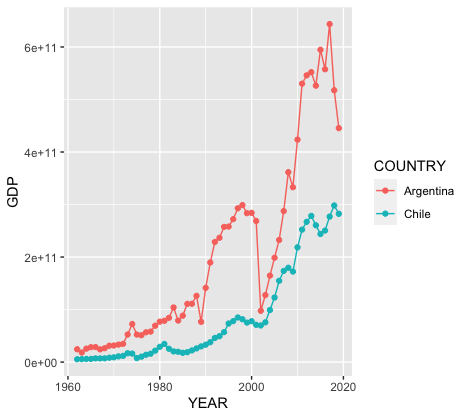
\includegraphics{GDP Plot.png}
\caption{Scatter Plot of GDP Observations by Country 1962-2019}\citet{WB:2021}
\label{fig:fig1}
\end{figure}

%----------------------------------------
% Figure 2
%----------------------------------------
\begin{figure}[ht]
\centering
\bigskip{}
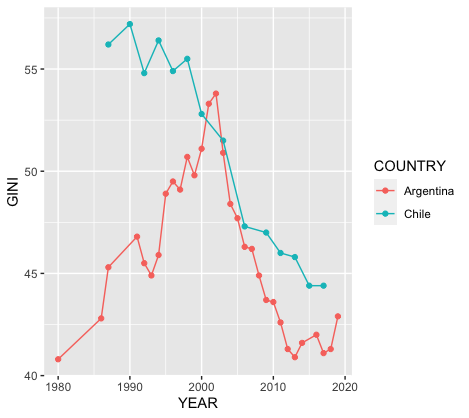
\includegraphics{GINI Plot.png}
\caption{GINI Index Observations by Country 1980-2019}\citet{WB:2021}
\label{fig:fig2}
\end{figure}


%----------------------------------------
% Table 1
%----------------------------------------

\begin{table}[!htbp] \centering 
  \caption{} 
  \label{} 
\begin{tabular}{@{\extracolsep{5pt}}lc} 
\\[-1.8ex]\hline 
\hline \\[-1.8ex] 
 & \multicolumn{1}{c}{\textit{Dependent variable:}} \\ 
\cline{2-2} 
\\[-1.8ex] & GDP \\ 
\hline \\[-1.8ex] 
 TIME & 216,824,729,956.000$^{***}$ \\ 
  & (43,126,076,569.000) \\ 
  & \\ 
 GROUP & $-$20,206,883,389.000 \\ 
  & (54,902,216,705.000) \\ 
  & \\ 
 DID & $-$122,632,825,911.000$^{**}$ \\ 
  & (60,989,482,377.000) \\ 
  & \\ 
 Constant & 27,896,670,724.000 \\ 
  & (38,821,729,734.000) \\ 
  & \\ 
\hline \\[-1.8ex] 
Observations & 116 \\ 
R$^{2}$ & 0.330 \\ 
Adjusted R$^{2}$ & 0.312 \\ 
Residual Std. Error & 128,757,111,240.000 (df = 112) \\ 
F Statistic & 18.354$^{***}$ (df = 3; 112) \\ 
\hline 
\hline \\[-1.8ex] 
\textit{Note:}  & \multicolumn{1}{r}{$^{*}$p$<$0.1; $^{**}$p$<$0.05; $^{***}$p$<$0.01} \\ 
\end{tabular} 
\end{table} 



\end{document}
